\chapter{Related Works}\label{ch:related}

This chapter presents relevant work in the area of \gls{mot} and age and gender recognition.

\section{\glsentrylong{mot}}

% what is MOT
\glsentrylong{mot} is a longstanding goal in computer vision\cite{zhang2020fair, Bewley_2016_SORT, MOT16}, which aims to estimate trajectories for objects of interest in videos.

% Tracking-by-detection as the preferred algorithm - two-step process
Tracking-by-detection has emerged as the preferred paradigm to solve the \gls{mot} problem\cite{MOT16, Wojke2017_DeepSORT}. This paradigm simplifies the task by breaking it into two steps: detecting the objects' locations independently in each frame and then forming tracks by associating corresponding detections across time. The second step is sometimes called linking or \gls{reid}.

% CNN as detectors are the way to go
In recent years,  \gls{nn}  based  detectors  have  clearly outperformed all other methods for detection.\cite{ren2015fasterRCNN, yolo}. 

% associating tracks (ReID)
Track association has been handled by various methods. Straightforward \gls{iou}\footnote{\gls{iou} of two areas is the area of their overlap over the area of their union.} based approach has been applied\cite{bochinski2017high_IOUtracking} as well as various embeddings from \glspl{nn}\cite{Wojke2017_DeepSORT}. The association step usually first computes a cost matrix based on the motion and appearance information and then matches the tracks to minimize the total cost.

% two-step method advantages
When using the two-step method, one can develop the most suitable model for both tasks separately. Additionally, one can crop and resize the image patches based on the bounding boxes before estimating the \gls{reid} features.

% combining detection and ReID - FairMOT
Recently \cite{zhang2020fair} came up with a model that handles both the detection and \gls{reid} tasks while achieving accuracy comparable to \gls{sota} trackers.\cite{MOT16}

% end-to-end approach
An alternative approach using recurrent neural networks for data association has been explored in \cite{mot_with_rnn} and \cite{mot_with_longterm}. While providing some advantages, their work is not competitive with current \gls{sota} methods.\cite{MOT16}

\subsection{\glsentrylong{sort}}\label{s:sort}

% SORT
\Gls{sort} is a pragmatic approach to \gls{mot} with a focus on simplicity and performance introduced in \cite{Bewley_2016_SORT}, which uses Kalman Filter (introduced in section \ref{s:kalman}) to predict object location in the next frame. Cost matrix is based on \gls{iou}  of Kalman predictions and detections in the new frame. Finally, Hungarian algorithm\cite{kuhn1955hungarian} is adopted to make a minimum cost matching based on the \gls{iou}.

% SORT limitations
The main disadvantage of the \gls{sort} algorithm is its reliance only on position and movement data. This can easily lead to identity switches of tracks when occluded either by environment or by other tracks.

% DeepSORT
\Gls{deepsort} extends the \gls{sort} with appearance information from a \gls{cnn}.

To incorporate motion information \gls{deepsort} uses Mahalanobis distance between predicted Kalman states and newly arrived measurement:

$$
d^{(1)}(i,j) = (d_j - y_i)^T S_i^{-1}(d_j - y_i),
$$
where $(y_i, S_i)$ is the projection of the $i$-th track into measurement space and $d_j$ is the $j$-th bounding box detection. The Mahalanobis distance takes state estimation uncertainty into account by measuring how many standard deviations the detection is away from the mean track location. This metric makes it possible to exclude unlikely associations by thresholding the Mahalanobis distance. The threshold is calculated as a $95\%$ confidence interval computed from the inverse $\chi^2$ distribution.

To incorporate appearance information we compute an appearance descriptor $r_j$ for each detection $d_j$ with $||r_j|| = 1$. Furthermore, we keep a history $\mathcal{R}_k$ of the last $L_k$ descriptors for each track $k$. We then measure the distance between the $i$-th track and $j$-th detection as the smallest cosine distance:
$$
d^{(2)}(i,j) = \min\{1 - r_j^T r_k^{(i)}\; |\; r_k^{(i)} \in \mathcal{R}_i\}.
$$

We can also find a suitable threshold to indicate if an association is admissible according to this metric using a training dataset.

We can combine both motion-based information from Mahalanobis distance and appearance-based information from the cosine distance using a weighted sum
$$
c_{i,j} = \lambda d^{(1)}(i,j) + (1-\lambda)d^{(2)}(i,j),
$$
where we call an association admissible if it is admissible for both thresholds described above.

The influence of each metric can be controlled through the hyperparameter $\lambda$.

\subsection{Metrics}

To evaluate and compare different methods, we need a way to measure errors. While this is very straightforward for some tasks, this is not the case for \gls{mot}. \cite{bernardin2008evaluating_Clear_mot_metrics} introduces two relatively simple and intuitive metrics that will be described in this section. Both metrics are widely used\cite{MOT16}.

The first metric is called \gls{motp} and characterizes trackers precision in estimating object positions. The second metric is \gls{mota} and expresses the tracker's ability to determine correct object configuration and keep consistent tracks.

The procedure for calculating these metrics consists of three steps each frame:
\begin{enumerate}
    \item establish the best possible correspondence between hypotheses and objects,
    \item for each correspondence compute the error in objects position estimation,
    \item accumulate following errors:
    \begin{itemize}
        \item count all objects with no hypothesis as misses (\textit{false negatives}),
        \item count all hypotheses with no real objects associated as \textit{false positives},
        \item count all occurrences where the tracking hypothesis for an object changed compared to previous frames as \textit{mismatches}.
    \end{itemize}
\end{enumerate}

\begin{figure}[ht]
    \centering
    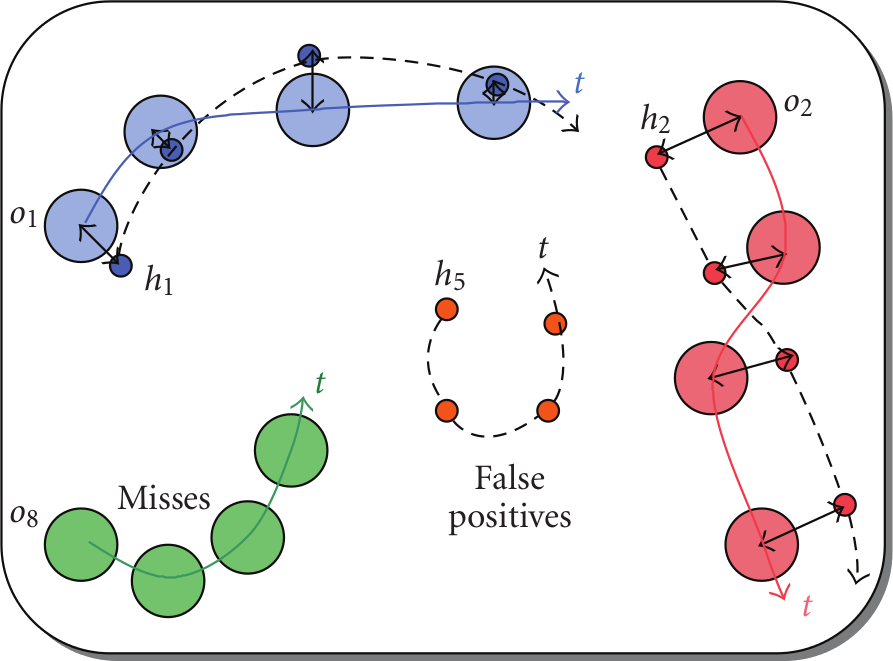
\includegraphics[width=8cm]{mot_errors}
    \caption[Illustration of various types of errors.]{Illustration of various types of errors.\cite{bernardin2008evaluating_Clear_mot_metrics}}
    \label{fig:mot_errors}
\end{figure}

Let $c_t$ be the number of matches for time $t$. For each match, let $d_t^i$ be the distance between the object and the hypothesis. The \gls{motp} is then defined as:

$$
\text{MOTP} = \frac{ \sum_{i,t}d_t^i }{ \sum_t c_t }.
$$

Let $m_t$ be the number of misses, $\mathit{fp}_t$ the number of false positives, $\mathit{mme}_t$ the number of mismatches and $g_t$ total number of objects in time $t$. The \gls{mota} is then defined as:

$$
\text{MOTA} = 1 - \frac{ \sum_t(m_t + \mathit{fp}_t + \mathit{mme}_t) }{ \sum_t g_t  }.
$$

The \gls{mota} can be seen as computed from three ratios - miss ratio, false positives ratio, and mismatch ratio.

For more discussion and implementation details see \cite{bernardin2008evaluating_Clear_mot_metrics}.

\section{Person Re-identification}\label{s:reid}

Person \gls{reid} is a fundamental task for people \gls{mot}. One person's appearance can change significantly in different frames, for example, by changing pose, turning around, or taking off a backpack. On the other hand, people often wear similar clothes and may look very similar, especially when viewed from a distance. These variations make the task challenging.

\cite{osnet} presents \textit{OSNet}, a \gls{cnn} architecture for tackling the \gls{reid} task. While \glspl{cnn} have been used before (for example in \cite{Wojke2017_DeepSORT}) to learn discriminative features for \gls{reid}, \textit{OSnet} presents a novel approach.

Key concept in \textit{OSnet} is focus on \textit{omni-scale} feature learning and its effective implementation. Authors argue that using even features at multiple scales (for example, local and global features) is not sufficient and features of all scales are crucial for the \gls{reid} task.

The result is a lightweight \gls{reid} network that achieves \gls{sota} results on multiple datasets outperforming even much bigger models.\cite{osnet}
